\documentclass[Main.tex]{subfiles} 
\begin{document}
\begin{figure}[H]%[htbp]
\centering
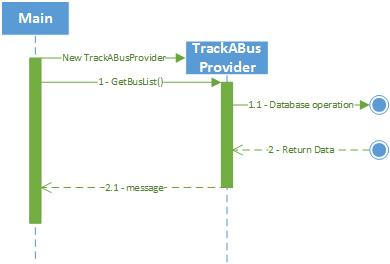
\includegraphics[scale=1.00]{Diagrammer/MainTrackABusThreadCom.jpg}
\caption{Sekvensdiagram over - Main og TrackABusProvider p� mobil applikationen}
\label{fig:SekvensdiagramTrackAbusThread}
\end{figure}
P� figur \ref{fig:SekvensdiagramTrackAbusThread} vises et eksempel p�, hvordan main tr�den i mobil applikationen kommuniker med TrackABusProvideren. TrackABusProvideren agerer som en BoundService, hvilket betyder, at det er muligt at kalde til den, i det �jeblik den er bundet. Den skal alst� ikke instantieres. En ny tr�d skabes, der kalder ned i data tilgangs laget for at hente data fra MySQL databasen, alt efter hvilken TrackABusProvider funktion, der er blevet kaldet. Det kan ses at main tr�den ikke bliver blokeret imens det hentes fra databasen. N�r TrackABusProvider er f�rdig med at hente data fra databasen, bliver der sendt en message til main tr�den, som indeholder det hentede data. Ved hj�lp af en message handler vil beskeden blive modtaget i main tr�den, og brugeren bliver pr�senteret for det hentede data.\\
SetFavoriteBusRoute og RemoveFavorite bliver blot startet af main tr�den, og sender en besked tilbage n�r de er f�rdige med at gemme eller slette fra SQLite databasen. Det vil ikke v�re muligt at starte en ny SetFavoriteBusRoute eller RemoveFavorite imens en af dem k�rer.
\end{document}